\section{Extreme-Token Phenomena Over Many Samples}\label{sec:many_samples}
In this section we show that the extreme-token phenomena, and our predictions from the BB model, exhibit in prompts other than ``Summer is warm. Winter is cold.'' To this end, we use 128 samples from the Wikipedia dataset, each truncated to 8 tokens. \Cref{fig:extreme_tokens_llama_31_many_samples} provides aggregate statistics of extreme-token phenomena in Llama 3.1-8B, which are similar to the fine-grained statistics over a single prompt from \Cref{figure:extreme-token}. \Cref{fig:extreme_tokens_olmo_many_samples} provides aggregate statistics of the development of extreme-token phenomena over the training dynamics of OLMo, which are similar to the fine-grained statistics over a single prompt from \Cref{fig:olmo_predictions_phase0} and \Cref{fig:olmo_predictions_phase1}.


\begin{figure}[h]
    \centering
    \begin{subfigure}{0.31\textwidth}
        \centering 
        \caption{Attention weights (L24).}
        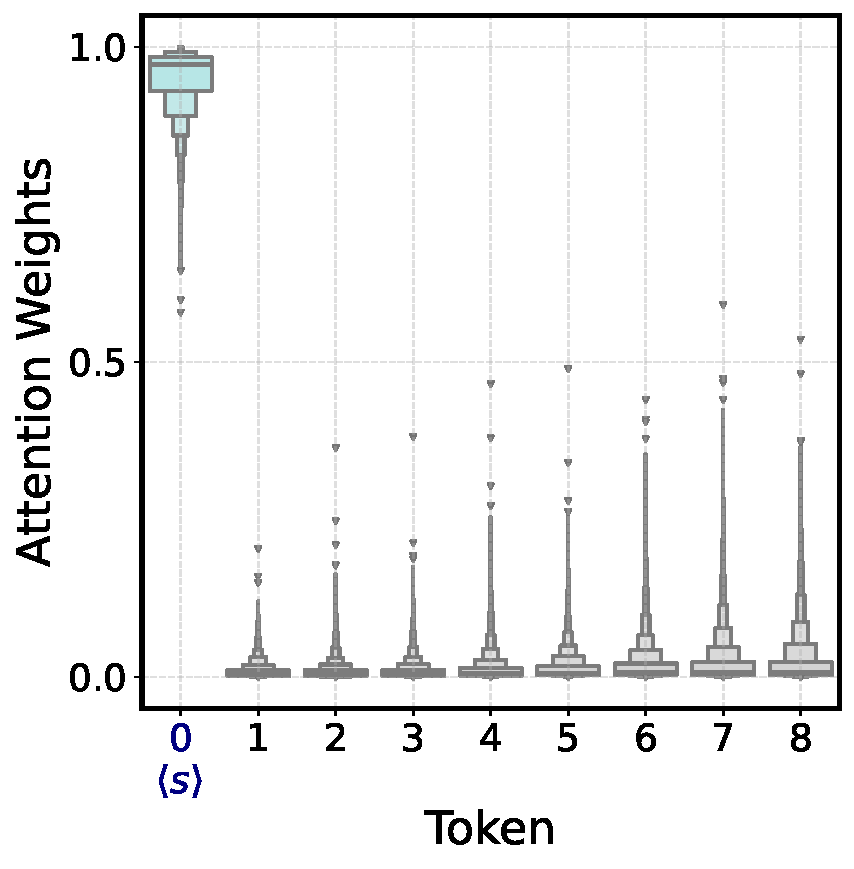
\includegraphics[width=\textwidth]{Figures/more_samples_statics/attn_weights_k_tokens.pdf}
    \end{subfigure}
    \hfill
    \begin{subfigure}{0.31\textwidth}
    \centering 
    \caption{Value state norms.}
    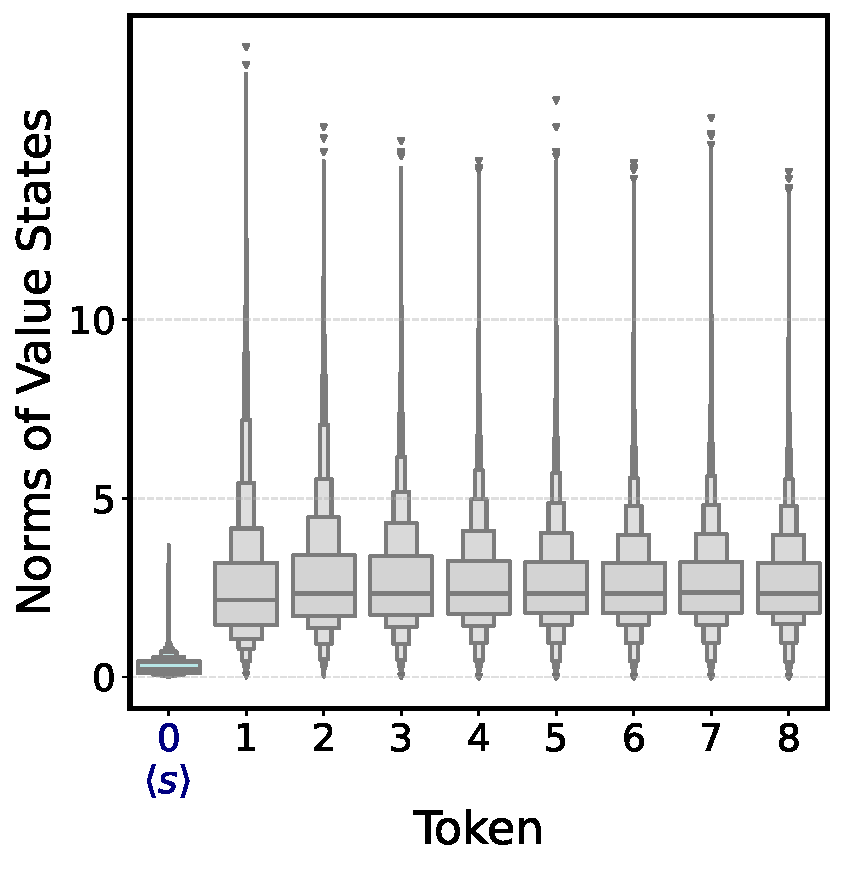
\includegraphics[width=\textwidth]{Figures/more_samples_statics/val_drain_batch.pdf}
    \end{subfigure}
        \hfill
    \begin{subfigure}{0.32\textwidth}
        \caption{Residual norms.}
        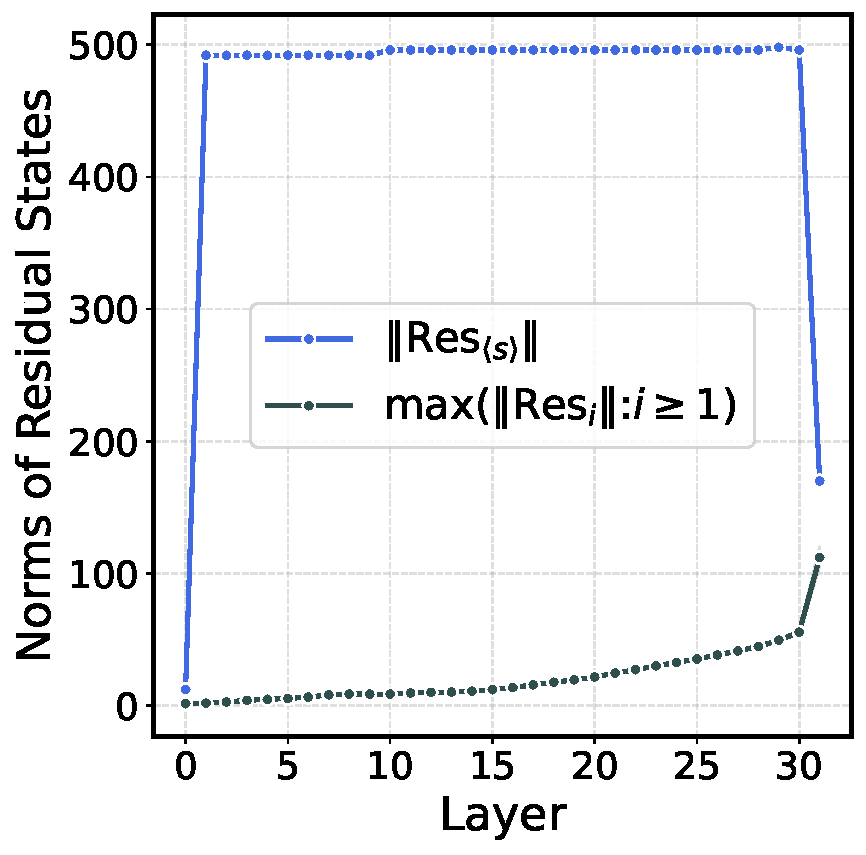
\includegraphics[width=\textwidth]{Figures/more_samples_statics/res_peak_batch.pdf}
    \end{subfigure}
    
    \caption{\textbf{Extreme token phenomena over many samples in Llama 3.1-8B-Base.} \textit{Left (a):} Let \(A\) be the attention weight tensor, of shape \((\text{batch size=128, \# heads=32, \# tokens=8, \# tokens=8})\) at Layer 24 of Llama 3.1-8B-Base. We calculate the tensor \(\bar{A}\), of shape \((\text{batch size=128, \# heads=32, \# tokens=8})\), which measures the average attention mass on the key tokens, by the following calculation: \(\bar{A}_{bhj} \doteq \frac{1}{n-j}\sum_{i = j}^{n}A_{bhij}\). We expect, for an attention sink head \(h\) on sample \(b\), that \(\bar{A}_{bh0}\) is large, and \(\bar{A}_{bhj}\) is small for all \(j \geq 1\). We indeed see this by plotting the distribution of \(\bar{A}_{:, :, j}\) for each \(j\), which shows that almost all attention mass is concentrated on the \bos token with high probability, showing the same thing as the individual attention head analysis in \Cref{figure:extreme-token} (a). \textit{Middle (b), Right (c):} We do the same computations as \Cref{figure:extreme-token} (b) and (c), averaged over the \(128\) samples.}
    \label{fig:extreme_tokens_llama_31_many_samples}
\end{figure}

\begin{figure}
    \centering
    \begin{subfigure}{0.45\textwidth}
    \centering 
    \caption{Attention weights (L24).}
    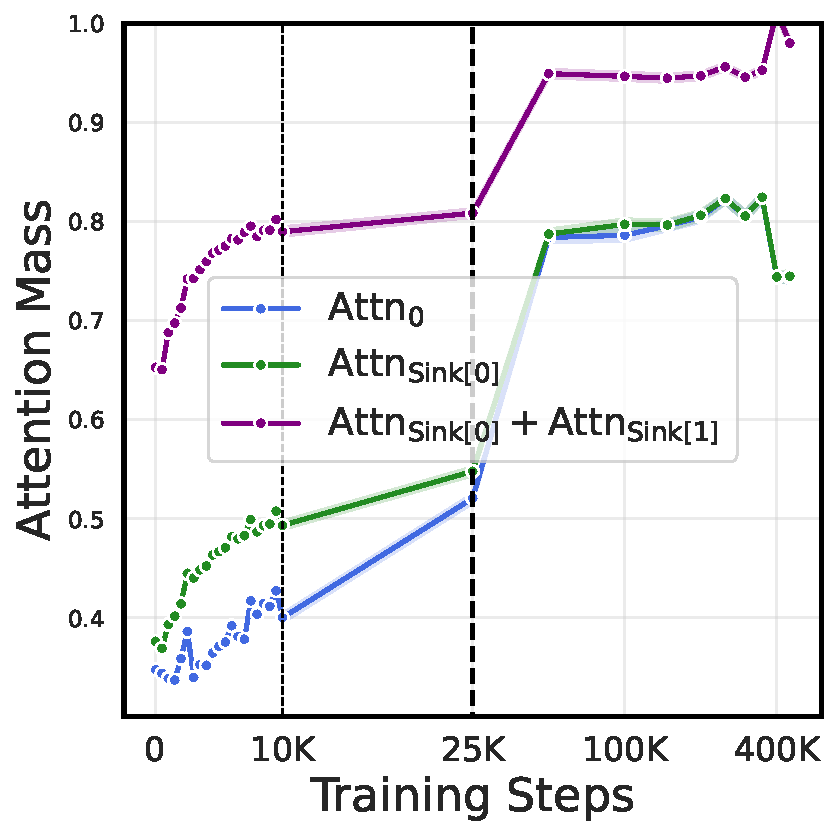
\includegraphics[width=0.7\textwidth]{Figures/olmo_batch/attn_mass_on_top_two_tokens.pdf}
    \end{subfigure}
    % \hfill
    \begin{subfigure}{0.45\textwidth}
    \centering 
    \caption{Attention logits (L24).}
    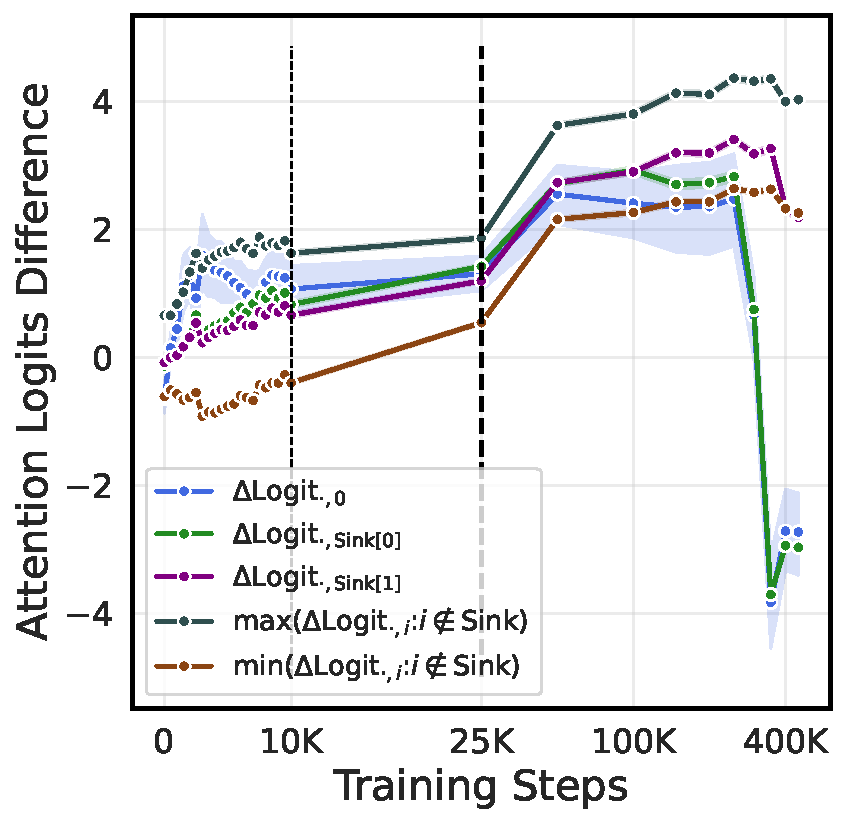
\includegraphics[width=0.7\textwidth]{Figures/olmo_batch/attention_logits.pdf}
    \end{subfigure}
    
    \begin{subfigure}{0.45\textwidth}
    \centering 
    \caption{Value state norms (L24).}
    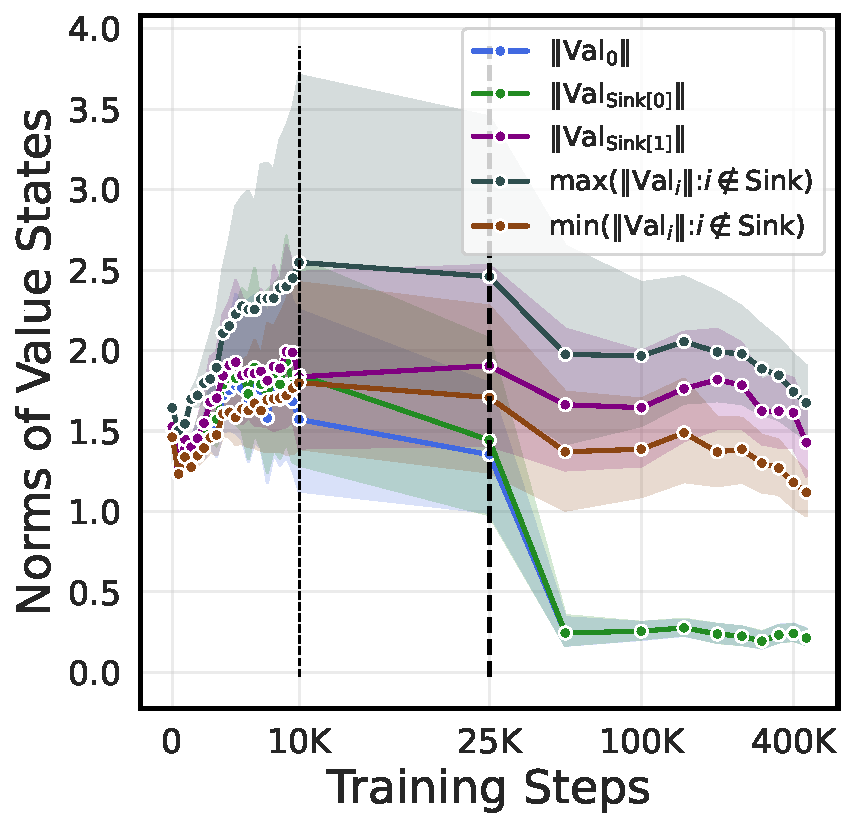
\includegraphics[width=0.7\textwidth]{Figures/olmo_batch/value_norms.pdf}
    \end{subfigure}
    % \hfill
    \begin{subfigure}{0.45\textwidth}
    \centering 
    \caption{Residual norms (L24).}
    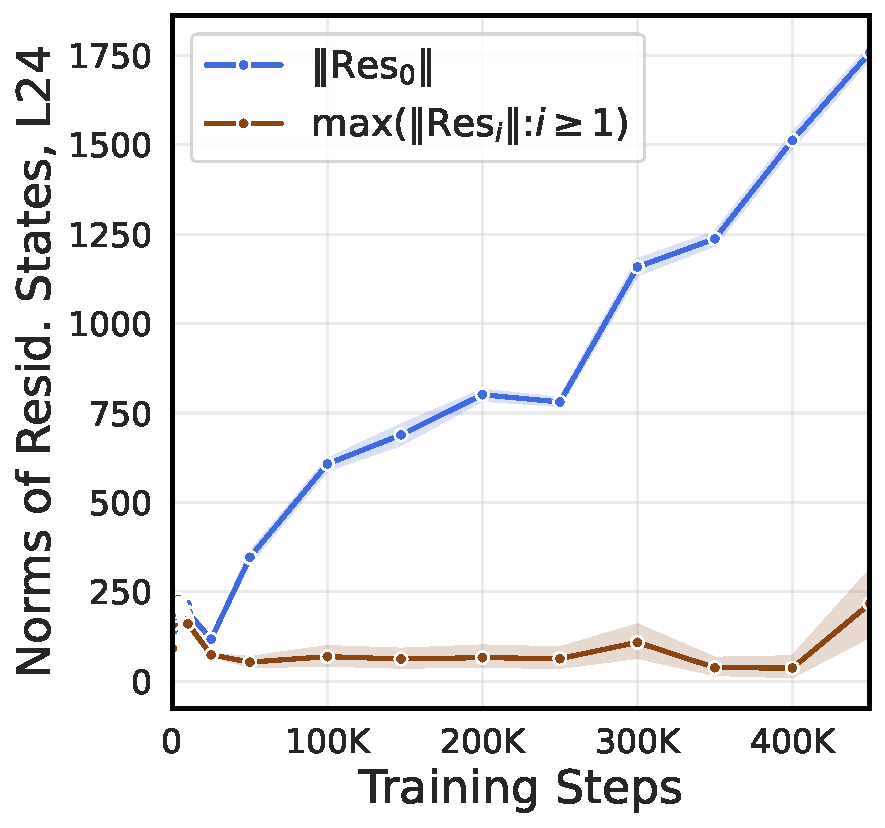
\includegraphics[width=0.7\textwidth]{Figures/olmo_batch/layer_output_norms.pdf}
    \end{subfigure}

    \caption{\small \textbf{Dynamics of extreme-token phenomena in layer 24 over many samples in the training trajectory of OLMo-7B.} For this experiment, as in \Cref{sub:olmo_dynamics}, for each sample and attention head we designate two attention sink tokens as the two tokens with the largest average attention mass \(\bar{A}_{bhj}\) (see \Cref{fig:extreme_tokens_llama_31_many_samples} for definition). We then study the dynamics of sink tokens versus non-sink tokens. In these experiments we observe that token \(0\) is (almost) always a sink token, which we discuss further in \Cref{sub:fixed_bos}. \textit{Top left (a):} The average attention scores \(\bar{A}_{bhj}\) for \(j\) as a sink token versus non-sink tokens. We observe that attention sinks form in nearly all heads and samples: the attention mass on top tokens nearly always sums to \(1\), and moreover the sinks develop relatively early in training. \textit{Top right (b):} We observe that the normalized attention logits of non-sink tokens initially increase until the formation of an attention sink, and then approximately converge to a stable phase with similar logits on token \(0\). \textit{Bottom left (c):} We observe that the value states of all tokens except the first sink token (token \(0\)) rapidly converges to steady state, while the first sink token has a much lower value state norm than all other tokens. \textit{Bottom right (d)}: We observe that the norm of the residual state of token \(0\) increases linearly during pretraining, while all other tokens' residual states do not. Our results mirror and confirm the single-sample detailed analysis conducted in \Cref{sub:olmo_dynamics}.}
    \label{fig:extreme_tokens_olmo_many_samples}
\end{figure}
